\chapter{État de l'art}
\section{Introduction}
\paragraph{}
Les bases de connaissances jouent un rôle de plus en plus important dans l'essor du Web. Ainsi, elles favorisent l'intégration de l'information qui enrichit le contenu du Web. La plupart des bases de connaissances contiennent des informations relatives à des actions dans le temps qui ne possèdent pas la bonne structure capable de relier directement l'événement au temps ou à la période associée à cet événement.
Ces bases de connaissances portent sur des domaines variés (les entreprises, les films, la musique, les livres, les publications scientifiques etc...) et sont créées par des ingénieurs de connaissance. 
\subparagraph{}
Notre étude s'appuie sur DBpedia, une source gigantesque de connaissances par l'extraction des informations structurées à partir de Wikipédia pour rendre ces informations plus utiles et également accessibles sur le Web. La base de connaissances DBpedia a plusieurs avantages sur les bases de connaissances existantes : elle est représentée en RDF et l'accès au dépôt de données se fait avec des requêtes sur la base de données via SPARQL. Elle couvre plusieurs domaines, évolue automatiquement avec les changements de Wikipédia, est multilingue et accessible sur le Web. 
Comme DBpedia couvre un large éventail de domaines et contient environ 4,8 milliards de triplets RDF qui couvrent des domaines divers, un nombre croissant d'éditeurs de données ont commencé à mettre des liens RDF à partir de leurs sources de données à DBpedia.
\subparagraph{}
Durant cette étude, nous avons travaillé sur les bases de connaissances pour annoter temporellement leurs contenus. Nous avons choisi praticulièrement DBpedia et nous avons développé un système automatique d'extraction d'informations qui convertit une partie du contenu de DBpedia dans une base de données temporelle riche et plus structurée que nous avons appelé SPOTBase.
\subparagraph{}
SPOTBase regroupe des triplets annotés générés automatiquement à l'aide d'une procédure de ``mapping'' que nous avons implémenté à partir de DBpedia.
Nous avons réussi à former environ $300$ quadruplets et beaucoup plus dans certains cas pour un seul couple de propriétés DBpedia qui valide bien notre hypothèse.
\subparagraph{}
Dans ce chapitre, nous introduisons les différents modèles, paradigmes et technologies que nous allons utiliser dans notre étude ainsi que les travaux de recherche liés à cette problématique, tout en analysant les différentes approches.
\section{Positionnement}
\paragraph{}
Notre étude a la particularité de vouloir enrichir le contenu du Web en utilisant l'extraction des données. 
En effet, nous utilisons les techniques d'extraction des données depuis les différentes sources d'informations pour les réinjecter plus tard dans le Web sémantique. Notre travail vise à enrichir la sémantique des triplets RDF dans les bases de connaissances avec des annotations temporelles.
\section{Problèmatique}
\paragraph{}
Lorsqu’on explore DBpedia, on trouve beaucoup de triplets qui décrivent des informations temporelles. Ces triplets sont généralement liés à un contexte événementiel précis.
Il est plus difficile d’exploiter ces informations si elles ne possèdent pas une structure universellement valide, claire et lisible par la machine. Dans DBpedia, il se trouve que des informations liées au même contexte temporel sont exprimées de la manière suivante : 
\begin{figure}[H]
        \centering
                \centering
                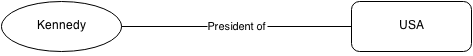
\includegraphics[width=10cm]{ken.png}
               \caption{triplet ''Kennedy''}

\end{figure}
\subparagraph{}
Le premier triplet n'a pas une sémantique valide que en tenant compte du triplet suivant~: 
\begin{figure}[H]
        \centering
                \centering
                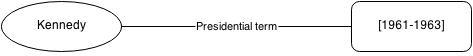
\includegraphics[width=10cm]{presidterm.png}
               \caption{triplet presidential term ''Kennedy''}

\end{figure}
\subparagraph{}
Plusieurs travaux de recherche ont proposé des différents syntaxes pour annoter des triplets RDF, mais ils ne donnent aucune indication sur la façon dont les annotations sont créées ou générées.
De plus, aucun algorithme n'a été proposé pour répondre à ce besoin.
Dans cette étude, on vise à annoter les triplets <$sujet$, $prédicat$, $objet$> avec une étiquette temporelle qui indique et précise la validité de ce triplet dans un cadre logique qui appartient au monde réel où en dehors de ce cadre, on peut dire que ce triplet RDF n'est pas valide et qu'on ne peut pas l'utiliser. Nous proposons une implémentation d'un système d'annotation sous forme d'une application Java et nous décrirons les résultats de notre système d'annotation.
\section{Technologies du Web sémantique}
\subsection{Intérêt du Web sémantique}
\paragraph{}
Le Web sémantique est un domaine de recherche né des travaux de Tim Berners-Lee et al.~\cite{Berners-lee2001}. Ces efforts ont pour but d'ajouter du sens aux contenus du Web et d'automatiser l'accès à l'information utile sur le Web. La question n’est pas d'ajouter une autre alternative au Web, il s’agit plutôt d'étendre le Web dans le but d'utiliser et de manipuler le maximum de son contenu informatiquement afin de permettre à des programmes informatiques de traiter un ensemble étendu de données issues du Web.
\subsection{Modèle RDF}
\paragraph{}
Au centre du Web sémantique, comme la brique de base qui permet d’ériger les plus grands édifices, se trouve le modèle {\itshape\gls{rdf}}. RDF~\cite{RDF_Concepts_W3C:04} est un standard de {\itshape \gls{w3c}} qui se base sur un modèle de graphe sous forme de triplets <$sujet$, $prédicat$, $objet$> : 
\begin{itemize}
\item Le sujet est identifié par un {\itshape \gls{iri}} ou peut être un n\oe{}ud anonyme.
\item Le prédicat est nécessairement identifié par un IRI.
\item L'objet peut être :
\begin{itemize}
\item Une ressource identifié par un IRI ou un n\oe{}ud anonyme.
\item Un littéral
\end{itemize}
\end{itemize}
Les triplets RDF permettent d'exprimer tous les types d'assertions. Il s’agit d’un cadre de description de ressources d’une façon formelle sur le Web. 
\subparagraph{}
C’est la première brique de standard du Web sémantique qui recouvre à la fois un modèle et plusieurs syntaxes pour publier des données variées sur le Web.
Dans RDF :
\begin{itemize}
\item Les ressources sont un concept de base du Web sémantique. Tout ce qui peut être référencé est une ressource. Dans un contexte plus technique, tout ce qui peut être identifié par un \gls{uri} / \gls{iri} peut être considéré comme une ressource.
\item Un ensemble d’attributs décrivent la ressource qui possède des caractéristiques et des relations avec d’autres ressources.
\item Le cadre standardise la syntaxe de ces descriptions, mais aussi les modèles et les langages.
\end{itemize}
\subparagraph{}
La plus petite structure de description en RDF est le triplet.
\begin{figure}[H]
\centering
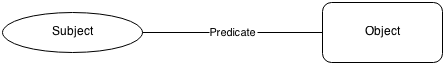
\includegraphics[width=8cm]{tripletrdf.png}
\caption{triplet RDF}
\end{figure}
\subparagraph{}
Un triplet décrit une ressource, l’associe à une propriété et à une valeur de cette propriété qui peut être une nouvelle ressource liée. 
\newline
Par exemple, ``Moncef a écrit une page QuadsRDF.html à propos des quadruplets RDF” peut être décomposée en deux triplets ayant comme sujet ``QuadsRDF.html”: <QuadsRDF.html, creator, Moncef> et <QuadsRDF.html, topic, QuadrupletsRDF>.
\newline
Par conséquent, les suivants <$sujet$, $prédicat$, $objet$>, c'est-à-dire les triplets RDF suivants peuvent être exprimés :
\begin{verbatim}
- <http://www.exemple.com/QuadsRDF.html>, <http://www.purl.org
/dc/terms/creator>, ``Moncef''.
- <http://www.exemple.com/QuadsRDF.html>, <http://www.exemple.
com/terms/topic>, <http://www.exemple.com/QuadrupletsRDF>.
\end{verbatim}
On peut schématiser cela de la manière suivante :
\begin{figure}[H]
\centering
\centering
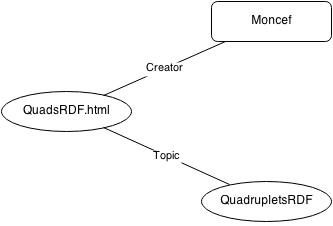
\includegraphics[width=8cm]{Diagram.png}
\caption{Deux triplets liés au même sujet}
\end{figure}
\subsection{Le langage de requête SPARQL}
\paragraph{}
Si RDF fournit un modèle universel de représentation de métadonnées, d'autres niveaux de traitements ont été standardisés au-dessus de lui et notamment l'interrogation de ces métadonnées. 
{\itshape \gls{sparql}}~\cite{SPARQL_W3C:13} fournit le langage d'interrogation du Web sémantique et il est à RDF ce que {\itshape \gls{sql}} est aux bases de données relationnelles.
\subparagraph{}
SPARQL est un langage d'interrogation de graphes RDF dont l'énoncé de base est lui aussi un triplet. Il est une recommandation du W3C depuis juillet 2008.
Poser une question en SPARQL consiste à écrire un graphe requête pour lequel on cherche des occurences dans le graphe cible.
\subsection{N-Quads}
\paragraph{}
N-Quads\footnote{http://sw.deri.org/2008/07/n-quads/} est un format qui s'étend N-Triples\footnote{http://www.w3.org/2001/sw/RDFCore/ntriples/} (une simple syntaxe pour les graphes RDF). Chaque N-uplet dans un document N-Quads peut avoir une valeur de contexte en option : <$sujet$, $prédicat$, $objet$, $contexte$>. La notion de provenance est essentielle lors de l'intégration des données provenant de différentes sources ou du Web. N-Quads est une recommandation W3C depuis $2014$.
\subsection{Ontologies}
\paragraph{}
La définition de référence d’une ontologie provient de Gruber~\cite{gruber1995} : {\it Une ontologie est la spécification d’une conceptualisation. [...] Une conceptualisation est une vue abstraite et simplifiée du monde que l’on veut représenter.} 
\subparagraph{}
\textbf{Exemple de vocabulaire RDF} On considère les relations suivantes : \textit{dc{:}title}, \textit{dc{:}author} et \textit{foaf{:}knows}, {\tt dc} et {\tt foaf} sont des préfixes relatifs à {\tt<http://purl.org/dc/elements/1.1/>} et {\tt<http://xmlns.com/foaf/0.1/>}. Celles-ci ont été définies dans les vocabulaires Dublin Core\footnote{http://www.w3schools.com/webservices/ws\_rdf\_dublin.asp} et FOAF\footnote{http://xmlns.com/foaf/spec/}. Un vocabulaire modélise un domaine particulier : concepts, relations. Par exemple FOAF modélise les personnes et leurs relations entre elles. Il identifie les classes $Person$, $Agent$, $Organisation$, etc. et les relations \textit{firstName}, \textit{familyName}, \textit{knows}, \textit{birthday}, etc. Le vocabulaire structure ensuite ces  éléments : \textit{Person} est une sous-classe de \textit{Agent}, \textit{familyName} a pour domaine la classe \textit{Person}, etc.
\subparagraph{}
\textbf{RDF Schema, ou RDFS}~\cite{RDF_Schema_W3C:04}, est le langage de description de vocabulaire historiquement associé à RDF. Il s'agit en effet du premier des langages de description de vocabulaire développés pour le Web de données. RDFS permet de spécifier des ontologies dites légères, c'est-à-dire de nommer des classes et des propriétés, de donner la signature de ces propriétés et de définir une organisation hiérarchique de ces classes et propriétés.
\subparagraph{}
\textbf{\gls{owl}}~\cite{OWL_Overview_W3C:04}, est un langage de définition d'ontologies pour le Web sémantique. Il est beaucoup plus expressif que RDF Schema. OWL permet d'exprimer les notions d'équivalence de classes ou de propriétés, d'égalité de ressources, de différence, de contrainte... OWL $1$ est une recommandation du W3C depuis $2004$.
\newpage
\subsection{Bases de connaissances}
\paragraph{}
Une base de connaissances regroupe des informations structurées, sous un format exploitable par un ordinateur. Elle peut contenir des règles, des faits ou d'autres représentations. Les bases de connaissances regroupent des informations structurées. C’est dans ce contexte que nous cherchons à exploiter ces informations pour les mettre dans une nouvelle structure qui englobe le temps.
\subsubsection{DBpedia}
\paragraph{}
Wikipédia est une encyclopédie en ligne et construite en mode participatif.
Les articles de Wikipédia sont constitués de : texte structuré, informations structurées, infobox, images, liens externes etc. (autant vers d'autres pages Wikipédia que vers le Web) et les informations les plus significatives sont présentées dans des cadres à part voir figure 3.1. 
DBpedia\footnote{http://wiki.dbpedia.org/Interlinking}~\cite{lehmann2014} est un projet universitaire et communautaire d’extraction et d’exploitation automatiques des données à partir de Wikipédia et les transforme dans une base de connaissances en RDF sous forme d'un graphe avec des entités reliées.
\begin{wrapfigure}{r}{0.7\textwidth}
\vspace{-15pt}
\begin{center}
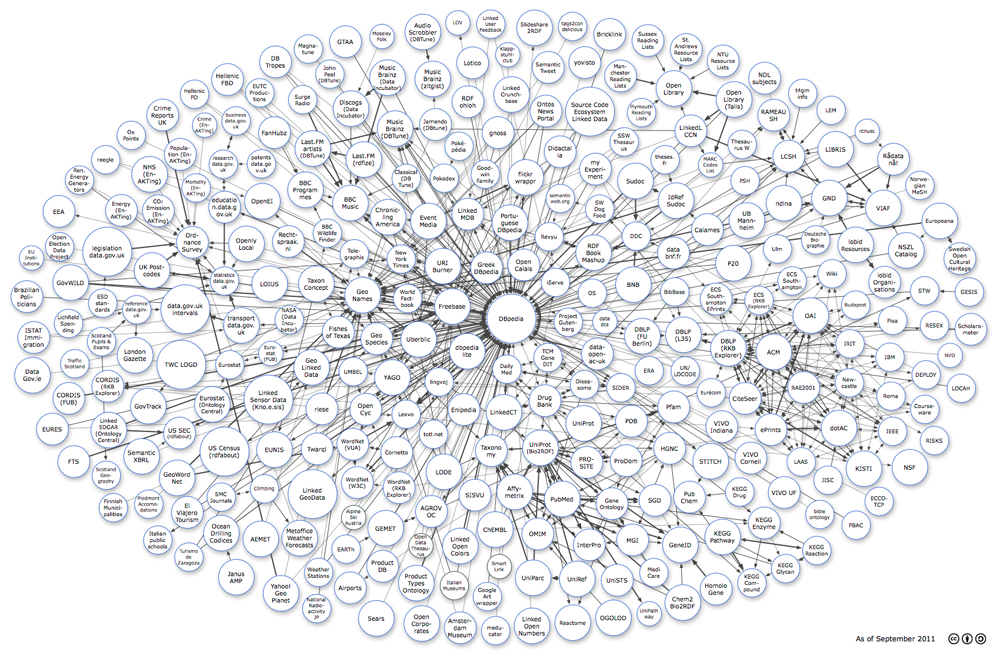
\includegraphics[width=0.50\textwidth]{dbpedia.png}
\end{center}
\vspace{-15pt}
\caption{DBpedia}
\vspace{-10pt}
\end{wrapfigure}
DBpedia 3.9 est la dernière version de DBpedia datant de Juin 2013.
Elle adopte les normes du Web sémantique et du réseau Linked Open Data. Pour chaque document encyclopédique, il existe une page de ressources contenant toutes les données et leurs descriptions sous forme de triplets RDF. Ces triplets peuvent représenter une information telle que ``Obama est le président des État-Unis''.
DBpedia est conçu par ces auteurs comme l'un des noyaux du Web émergeant sous le nom de Web de données. Les triplets de cette base de connaissances représentent des faits du monde réel. DBpedia est une base de connaissances open source écrite en Scala et Java.
\newpage
\subsubsection{Architecture d'extraction de DBpedia}
\paragraph{}
DBpedia décrit plus que $3,4$ millions d'entités. Cette base de connaissances définit un identifiant global et unique qui peut être déréférencé sur le Web dans une riche description RDF de l'entité, des définitions et descriptions lisibles dans $119$ langues, la relation avec d'autres ressources, la classification à quatre hiérarchies de concepts, des faits divers liées à d'autres sources de données sur le Web. Ceci permet à DBpedia d'être un pôle central d'interconnexion pour le Web de données.   
\begin{figure}[H]
\centering
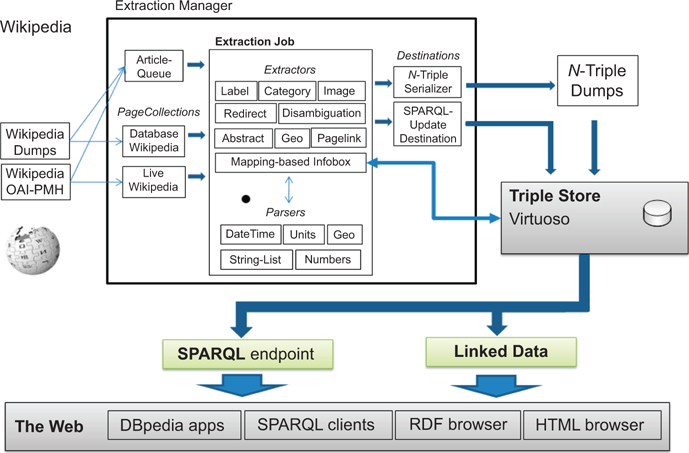
\includegraphics[width=12cm]{dbpediaExtra.png}
\caption{Extracteur DBpedia}
\end{figure}
La figure ci-dessus~\cite{morsey2012} montre l'architecture du système d'extraction des connaissances dans DBpedia.
D'apres Morsey et al~\cite{morsey2012} les principaux éléments du système sont les suivants : $PageCollections$ est une abstraction des ressources locales ou distantes des articles de Wikipédia, $Collections$ stokent ou sérialisent les triplets RDF extraites, $Extractors$ qui transforme un type spécifique de la syntaxe wiki en triplet, $Parsers$ soutiennent les $Extractors$ en déterminant les types de données, convertit les valeurs entre différentes unités et fractionne les marqueurs dans des listes. L'$Extraction$ $Job$ regroupe une collection de pages, extracteurs et destination dans le flux de travail $workflow$.
Le noyau de ce système est l'$Extraction$ $Manager$ qui gère le processus  d'adoption des articles de Wikipédia sur les $Extractors$ et donne les résultats à la destination.
Le gestionnaire d'extraction $Extraction$ $Manager$ gère également la gestion des URI et résoud les redirections entre les articles : ce système se compose de $11$ extracteurs qui traitent les types des contenus de Wikipédia {\tt(Labels, Abstracts, Interlanguage links, Images, Redirects, Disambiguation,
External Links, Pagelinks, Homepages, Categories, Geo-coordinates)}.
Ce framework d'extraction DBpedia est mise en place pour réaliser deux flux : extraction à partir des sources de données {\tt(DataBaseWikipedia page collections)} et une procédure d'extraction directe
{\tt(LiveWikipedia page collections with the OAI-PMH protocol)} pour obtenir la version courante des articles. Notre point d'accès à ce système d'extraction, plus précisément à la base RDF {\tt Triple Store} sera à travers des requêtes SPARQL. 
\subsubsection{YAGO}
YAGO\footnote{http://www.mpi-inf.mpg.de/yago-naga/yago/} est une large base de connaissances sémantiques, dérivrée de Wikipédia, WordNet\footnote{http://wordnet.princeton.edu/} et GeoNames\footnote{http://www.geonames.org/}. Actuellement elle contient plus de $10$ millions d’entités (personnes, organisations, villes, etc..) et plus de $120$ millions de faits au sujet de ces entités.
\newline
Les caractéristiques principales de YAGO :
\begin{itemize}
\item YAGO combine la taxonomie propre de WordNet avec la richesse du système de catégorie de Wikipédia, l'attribution des entités à plus de $350~000$ catégories.
\item YAGO est une ontologie qui attache une dimension temporelle et spatiale à plusieurs de ces faits et entités.
\end{itemize}
\subsubsection{Wikidata}
\paragraph{}
Wikidata est un projet de base de connaissances éditée d'une manière collaborative pour aider à la mise à jour des données de Wikipédia. Ce projet est lancé par Wikimedia Deutschland\footnote{https://www.wikimedia.de/wiki/Hauptseite}. Wikidata est déstiné à fournir une source commune de données objectives ou factuelles telles que les dates de naissances ou bien le PIB des pays, qui pourront être utilisées dans tous les articles des différentes versions linguistiques de Wikipédia, une mise à jour de Wikidata  pouvant être alors répercutée automatiquement sur l'ensemble des wikipédias en différentes langues. 
\section{Présentation du Linked Open Data}
\subsection{Données ouvertes}
\paragraph{}
 L'ouverture des données désigne un ensemble de mouvements technologiques, culturels et politiques visant à mettre à disposition certaines données pour permettre leur libre accès, sans restriction de copyright, brevet, licence payante ou autre.
L'ouverture des données permet en effet de construire des applications innovantes basées sur l'exploitation de ces données, d'effectuer des analyses de ces données et de conduire des travaux de recherche exploitant ces données.
\subsection{Données liées}
\paragraph{}
Le Web des données (Linked data ou Web of Data en anglais) désigne non seulement la mise sur le Web de données mais surtout leur mise en relation pour constituer un réseau global de données où, à partir d'une donnée, on accède aux autres données liées du Web. La clé de voûte du Web de données est le Standard URI qui désigne tout objet ou concept décrit. Dans le Web de données les relations sont entre URI, ce qui permet le partage de ces descriptions entre machines et leur interrogation automatique.
\subparagraph{}
L'appellation ``données ouvertes liées'', met l'accent sur l'opportunité qui nous est offerte d'exploiter les différentes sources du Web de données en les liant entre elles. 
\subsection{Linked Open Data}
\paragraph{}
{\bf\gls{lod}}\footnote{http://linkeddata.org/}, est un moyen de publier des données structurées sur le Web où les données contenues dans des bases de données sont exposées avec leur sémantique, ce qui donne la possibilité aux métadonnées d'être connectées et enrichies d'une manière solide, et permet également d'avoir plusieurs représentations d'un même contenu et de faire des rapprochements entre des ressources connexes. DBpedia fait partie du LOD et les données portent sur plusieurs domaines (Media, Géographie, Gouvernement, Publications, etc.).
Le Web de données a développé dans une grande fusion, de divers ensembles de données provenant de plusieurs domaines. Le LOD décrit les ressources identifiées par des \gls{uri} en représentant leurs propriétés et des liens vers d’autres ressources. L'ensemble des données fournit des connaissances du monde réel.
\section{Utilité des annotations}
\paragraph{}
En générale, l'annotation, consiste dans le rajout d'une ou des informations supplémentaires ; c'est une étiquette qu'on ajoute à une ressource Web. Depuis la création du Web, plusieurs systèmes d'annotation sont apparus (ThirdVoice, PageSeeder, HyperNews, Nestor, etc.).
Nous citons brièvement les conséquences liées à ces systèmes d'annotation sont : l'information annotée doit d'une manière ou d'une autre être structurée, utilisable et descriptive de la ressource ou de son utilisation. De plus, la ressource en question doit exister et peut être exploitée sur le Web indépendamment des informations qui lui sont associées. La figure ci-dessous montre le système intermédiaire entre le client et le serveur Web dans lequel il y a le service de gestion des annotations, permettant la communication entre ces deux entités.
\begin{figure}[H]
\centering
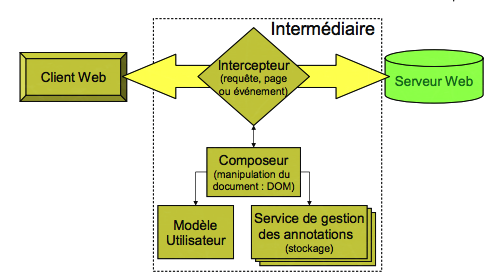
\includegraphics[width=14cm]{AnnotationSys.png}
\caption{Système de notation d'intermédiaire}
\end{figure}
\subparagraph{}
L'annotation sémantique faite référence à plusieurs types distincts d'annotations formelles, explicites et permanentes. Il existe des outils d'annotation basés sur les ontologies {\it Ontology based annotation tool}
et des critères relatifs aux annotations, par exemple : les types de ressources concernées, la structuration des schémas de description, l'automatisation marquée de la mise en place, etc.
\begin{figure}[H]
\centering
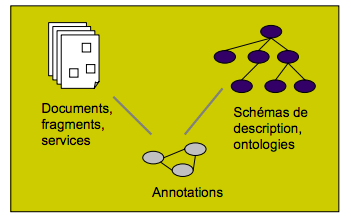
\includegraphics[width=9cm]{diffConnaissances.png}
\caption{Différents niveaux de connaissances}
\end{figure}
\subparagraph{}
L'annotation d'un triplet RDF est une façon d'ajouter des metadonnées à ce triplet pour décrire une restriction spatiale.
\newline
\textit{Comment on utilise les annotations ?} Un exemple d'utilisation est sur la plateforme ``sig.ma''\footnote{http://sig.ma/} crée par l'institut de recherche irlandais \textit{the digital enterprise research institute in Ireland (DERI)} spécialisé dans le domaine du Web sémantique et les données liées. La plateforme fournit un moteur de recherche par mot clé qui permet de récupérer des images et des textes accessibles par des annotations RDF, ainsi qu'une liste d'URI correspondant à la clé de recherche et des liens vers des ressources Web contenant des données RDF pertinentes.
\subparagraph{}
Dans le domaine du Web sémantique, plusieurs extensions de RDF ont été proposées pour exprimer le flou, la verité, la confiance, la certitude ou le temps.
Par exemple, pour la verité de certains triplets, on ajoute une valeur qui est entre $0$ et $1$, l’instance “Rome est une grande ville de degré 0.8” peut être représentée par $(Rome, type,grande{\_}ville) : 0.8$.
\subparagraph{}
De même pour la certitude, une autre forme a été proposé :
\newline
$(Max,hasSupervisor : (0.9,2003),William)$ à la forme générale suivante $(s, p : (x,t),o)$.
Dans ce dernier exemple, on remarque que l'annotation est sous forme de couple $(x, t)$ où $x$, la certitude, est représentée sous forme d'un pourcentage 90\% et $t$ le temps sous forme d'une année $2003$.
\section{Usage du traitement automatique des langues}
\paragraph{}
Le traitement automatique de la langue (TAL) est une discipline à la frontière de la linguistique, qui est intimement liée à l'intelligence artificielle.
On distingue plusieurs domaines d'application de TAL comme la traduction automatique, la génération automatique de texte, la correction orthographique, la reconnaissance de l'écriture manuscrite, etc.
Dans le cadre des annotations temporelles on pourrait utiliser les TAL.
\subsection{Les TAL pour l'ambiguïtés temporelles}
\paragraph{}
 Ambiguïtés temporelles est la propriété d'un mot ou d'une suite de mots qui peuvent avoir un ou plusieurs sens d'analyses grammaticales possibles. Dans une phrase simple ou composée, l'indicateur temporel peut avoir plusieurs sens selon le contexte de la phrase. Les informations temporelles peuvent avoir des représentations différentes~: 
\begin{itemize}
\item Un événement ``Je vous propose un rendez-vous $demain$ pour parler de ma plate-Forme PiSharing''. \item Une connaissance ``Jacques Chirac est le président de la république Française'' \textbf{ mais quand ?}
\end{itemize}
\subparagraph{} 
Le présent par exemple peut avoir plusieurs sens ou contextes : présent de narration, présent de généralité, présent qui réfère au futur proche, etc.
Les signaux temporels sont ambigus par exemple dans ces expressions : il court pour rattraper le temps, tu tournes après la rivière, etc. On remarque qu'il y a des indicateurs temporels, mais ce n'est pas le temps qui est relatif à un événement qui peut nous intéresser.
\paragraph{}
La plupart des expressions sont floues comme : il y a deux ans, toutes les deux semaines, j’arrive dans deux secondes, etc. En effet, il n'y a pas une logique descriptive qui peut nous aider à mettre un lien entre l'événement et la période temporelle. L’analyse du temps s’inscrit dans la compréhension globale des textes, et des événements auxquels on fait référence dans ce texte non pas en analysant une phrase comme suit. 
\newline
Modalité~: ``l’équipe de France voulait gagner la coupe du monde en 2014.'' 
\newline
Anaphore~:  ``..., cela pourrait avoir lieu dans les éditions suivantes.''
\subparagraph{}
Les événements décrits (et que l’on souhaite fixer temporellement) peuvent être : duratifs ou ponctuels/accomplis ou inaccomplis. 
De même pour les dates qui peuvent être des dates absolues ``$18$ mars $1990$, c'est ma date de naissance'' ; ou bien des dates relatives par rapport au moment de l’énonciation par exemple : ``il y a deux ans''. Pour la durée aussi on distingue plusieurs types comme la durée absolue ``durant 2 ans'' et la durée relative ``depuis un an''. Dans un texte, on trouve aussi un ensemble d'expressions de fréquence comme ``tous les ans, le vendredi 13'' et des expressions plus complexes comme ``après la Révolution Tunisienne''.
\subparagraph{}
Les textes contiennent des informations temporelles de taille massive qui sont difficilement exploitables. Nous avons donné une vue globale sur cette procédure qui peut être utile dans notre étude.
\subsection{Exploration des historiques des modifications dans Wikipédia}
\paragraph{}
L'historique des modifications dans Wikipédia est une page attachée à un article encyclopédique pour conserver le journal des modifications qui ont été apportées à cet article. Cette page permet de connaître la date, l'auteur et la teneur externe de chaque modification.
Dans cette encyclopédie, nous avons remarqué qu'à partir de l'historique de modifications, on peut déduire plusieurs informations liées à deux ou plusieurs contextes temporels différents.
Nous souhaitons, si c’est possible, extraire ces informations temporelles et les rendre exploitables dans DBpedia.
\begin{figure}[H]
\centering
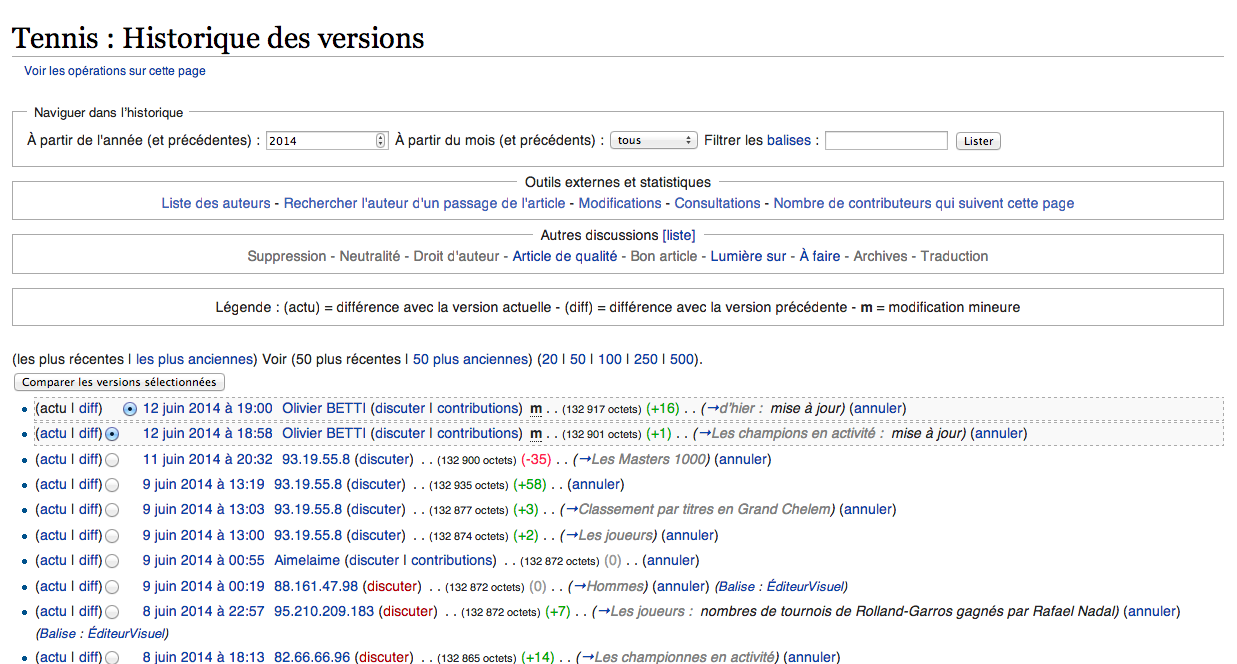
\includegraphics[width=11cm]{NEWHISTORIQUE.png}
\caption{Historique d'articles Wikipédia}
\end{figure}
\subparagraph{}
Cette partie impose une petite partie de TAL et ne peut s'appliquer que sur des faits récents.
\section{Différentes approches d'annotation temporelle}			
\paragraph{}
La nécessité de l’annotation temporelle sur les documents Web a été évoquée dans des nombreux travaux de recherche. La première approche formelle au problème de modélisation et d’interrogation temporelle en RDF a été introduite par Gutierrez et al.~\cite{gutierrez2005}.
\subparagraph{}
Ensuite, Udrea et al.~\cite{udrea2006} ont travaillé sur la notion d'annoter temporellement les graphes RDF et depuis d'autres travaux de recherche ont évoqué cette problématique.
Ces derniers définissent le triplet annoté de la forme suivante $(s,p:t,o)$ où $t$ est une étiquette temporelle. Cette notation a servi ensuite à formaliser des algorithmes pour interroger les données RDF annotées.
\subsection{RDF Temporel ou tRDF}
\paragraph{}
Pour introduire \gls{trdf}, on commence par les exemples suivants (Il y a des triplets comme par exemple : ``Mary est toujours la mère de John'' qui n'ont pas une caractéristique temporelle explicite parce qu’ils sont toujours valide. Mais il y a aussi des triplets ayant une valeur vraie que dans une plage temporelle bien précise, par exemple : ``Bill Clinton est le président des États-Unis", n'est valide que dans l'intervalle $[1993-2001]$).
\paragraph{}
Dans Pugliese et al.~\cite{pugliese2008} utilisent du temps discret, l’annotation tRDF est exprimée de la manière suivante ($n$ est un nombre entier, $T$ est un intervalle de temps, $s$ le sujet, $p$ le prédicat, $v$ l'objet) :
\begin{enumerate}
\item ($s$, $p$ : {$T$}, $v$), ce type de triplet représente une relation entre le sujet et le prédicat et l'objet dure un temps $T$ (dans n'importe quel point de temps dans $T$).
\item ($s$, $p$ : <$n$ : $T$>, $v$), ce triplet présente une relation entre $s$, $p$ et $v$ qui dure au moins $n$ point de temps différents dans $T$.
\item ($s$, $p$ : [$n$ : $T$], $v$), ce triplet présente une relation entre $s$, $p$ et $v$ qui dure au plus $n$ points de temps différents dans $T$.
\end{enumerate}
\subparagraph{} 
Divers représentations de l'annotation temporelle des triplets RDF ont été proposées. Nous avons remarqué une similarité entre eux ainsi : ($s$, $p$ : {$T$}, $v$) et ($s$, $p$, $v$): $T$ qui sont équivalents sémantiquement.	
\subsection{L'importance de l'annotation temporelle dans le Web de données}
\paragraph{}
Les raisonnements temporels d'informations ont besoin d'avoir la protée temporelle des faits tels que ``Mario Balotelli joue pour l'équipe AC Milan''.
Une approche a été proposée pour détecter la portée des événements visés par des triplets RDF par Rule et al.~\cite{rula2014}. Elle est composée de quatre étapes principales~:
\begin{itemize}
\item Les données d'un document Web sont normalisées pour tenir compte de l’importance des dates figurants dans ce document.
\item La sortie d'une phrase dans un document Web est comparée avec un ensemble d’intervalles de temps pertinents.
\item Un ensemble d’intervalles plus importants est sélectionné.
\item Les intervalles sélectionnés sont fusionnés.
\end{itemize}
\subparagraph{}
La plateforme DeFacto (Deep Fact Validation)~\cite{lehmann2012} a été utilisée pour la validation des états en cherchant des sources qu'elle confirme sur le Web.
Les triplets sont représentés par des faits et peuvent être associés à un contexte temporel.
Par exemple, $<Balotelli, team, AC Milan>$ se réfère à un événement de [$2003-2009$], une annotation temporelle est rattachée au fait comme suit $<f, [ti,tj]>$.
Cette approche combine deux types d'informations~: les informations temporelles recueillies dans des documents Web et les informations temporelles contenues dans les bases de connaissances, pour associer des intervalles de temps aux triplets RDF.
\subsection{Temps valide des triplets dans les données géospatiales liées}
\paragraph{}
Bereta et al.~\cite{bereta2013} introduisent la composante temporelle des données du modèle {\itshape\gls{strdf}} et le langage de requêtes {\itshape\gls{stsparql}}, pour la présentation et l’interrogation des données géospatiales liées qui changent dans le temps.
\subparagraph{}
L’introduction du temps dans les modèles de données et les langages de requêtes a été l’objet de recherches approfondies dans le champs des bases de données relationnelles.
\newline
Les trois types distincts de temps qui ont été étudiées~:
\begin{itemize}
\item L'action temporelle indépendante, par exemple ($01/12/1954$ c’est l’anniversaire de John).
\item Le temps d’événement ou un fait vrai dans l’application ( John a été professeur entre [$2001-2012$]).
\item Le délais de transaction est le moment où un fait est en cours dans la base de données (l’heure système $h$ présente l’heure exacte quand John est un professeur [$2001-2012$]).
\end{itemize}
\subparagraph{}
L’idée principale est d’intégrer les informations géospatiales pour le modèle de graphe RDF temporel. Le langage d’interrogation{ \it \gls{stsparql}\footnote{http://www.strabon.di.uoa.gr/stSPARQL}} ajoute deux nouveaux types de variables spatiales et temporelles aux variables SPARQL standards.
\subsection{Base de données temporelles}
\paragraph{}
Une base de données temporelle est une base de données avec des aspects de temps intégrés (temps-valide, temps-transaction), c'est-à-dire un modèle de données temporelles et une version temporelle du langage structuré de requête (SPARQL, SQL).
\subparagraph{}
En effet, le \textit{temps valide} dénote la période de temps durant laquelle un fait est vrai par rapport à la réalité.
Le \textit{temps-transaction} est la période de temps pendant laquelle un fait est stocké dans une base de données.
\paragraph{}
Dans le contexte de l'annotation temporelle des graphes RDF, les besoins se résument comme suit~:
\begin{itemize}
\item L'accès à différentes versions d’une ontologie.
\item Récupération des informations passées sur les sites Web.
\item La distribution des mises à jour des journaux.
\item Ajouter une étiquette à un triplet RDF pour exprimer sa validité temporelle.
\end{itemize}
\subparagraph{}
Antoniou et al.~\cite{antoniou2004} présentent une ontologie des services Web, pour montrer qu'une ontologie peut passer par plusieurs états dont l'objectif est d'analyser et de justifier les besoins cités auparavant.
\paragraph{}
Une base de données temporelle peut être exprimée comme un répertoire d'informations temporelles.
Gutiérrez et al.~\cite{gutierrez2007} montrent qu'il y aura deux manières pour ajouter des dimensions temporelles dans un graphe RDF intemporel~:
\begin{itemize}
\item Étiqueter les éléments soumis à des changements pour les triplets par exemple à chaque changement un nouveau 	 sera créé et l’ancien état sera stocké quelque part.
\item Versionner, c'est la capture du temps de transaction. D'après Gutiérrez et al.~\cite{gutierrez2007} l’étiquetage est mieux que les versions pour les raisons suivantes:
\begin{itemize}
\item Il conserve le principe de la nature distribuée et extensible de RDF.
\item Si la nouvelle version n’affecte que quelques éléments cela implique la création d’un nouveau graphe, de ce fait on aura des contraintes de mémoire et de stockage. 
\end{itemize}
\end{itemize}
\paragraph{}
Gutiérrez et al.~\cite{gutierrez2007} ont travaillé sur le domaine temporel à base de points et ont codé les points du temps en intervalle. Ces derniers ont proposé un vocabulaire pour affirmer les moments où les triplets sont valables dans un graphe RDF.
\section{Extraction des faits temporels}
\paragraph{}
L'extraction, la fouille de données, ou encore l'extraction de connaissances à partir de données, ont pour objet l'extraction d'un savoir, d'une connaissance, dans notre cas une connaissance mise en relation temporelle à partir de grandes quantités de données par des méthodes automatiques.
\subsection{Différentes approches de l'extraction }
\paragraph{}
Une approche proposée par Zweigenbaum et Tannier~\cite{zweigenbaum2013} consiste à détecter les relations temporelles entre les événements et les expressions temporelles à partir des comptes rendus hospitaliers.
La détection des relations temporelles entre les événements dans un texte fournit de bonnes informations pour l’extraction.
Dans TempEval Verhagen et al.~\cite{verhagen2010} ont abordé le temps dans un ``domaine ouvert” et cherchant à détecter en TempEval2 cinq types de relations temporelles :
\newline
$(Before, After, Overlap, Before\_or\_Overlap, Overlap\_or\_Before)$
Pour identifier les relations temporelles décrivant la chronologie du séjour hospitalier.
\newline
Les relations à trouver dans des différentes situations :
\begin{itemize}
\item{}Entre un événement et une date ou autre événement qui domine.
\item{}Entre un événement et la date de création de cet élément.
\item{}Entre deux événement principaux de deux phrases consécutives.
\end{itemize}
Identifier les informations temporelles décrivant la chronologie entre ces événements. Ces derniers utilisent des différents classifieurs (table de décision, arbre de décision, JRip, classifieurs bayésien naïf) et le classifieur à arbre de décision $J48$ implémenté dans weka\footnote{http://www.cs.waikato.ac.nz/ml/weka/}.
\subparagraph{}
La question est d’identifier les situations les plus importantes à traiter et les méthodes à utiliser pour cela.
Zweigenbaum et Tannier~\cite{zweigenbaum2013} utilisent une méthode d’apprentissage supervisée avec un ensemble de données et des classifieurs entrainés pour chaque situation.
L'évaluation a été appliquée sur un corpus d’apprentissage qui contient $190$ échantillons, dont $120$ échantillons de test. On peut utiliser cette méthode pour les propriétés de DBpedia à la place des comptes-rendus hospitaliers et chercher à chaque fois à apprendre à partir d'un motif qui peut être temporel, spatial, etc.
Au lieu d’une procédure de décision gloutonne ou aléatoire, une relation de décision globale pourrait être implémentée pour étudier toutes les relations temporelles prédites.
\paragraph{}
Dans un cadre différents, Kessler et al.~\cite{kessler2013} travaillent sur l'extraction des dates saillantes (importantes) qui méritent de figurer dans une chronologie événementielle.
Ces derniers ont utilisé une approche d’apprentissage pour extraire les dates saillantes concernant un thème donné. La méthode consiste à annoter automatiquement les informations événementielles. C’est-à-dire, à  repérer et à baliser les occurrences d’événements au sens TimeML~\cite{timml} ({\tt Time Markup language} est un langage d'annotation pour les événements et les expression temporelles) et de les classifier selon l’ontologie définie par le schéma d’annotation.
\subsection{Synthèse}
\paragraph{}
À présent que les principaux concepts ont été définis, mais aucune implémentation de ce système d'annotation n'a été proposée. Nous ne savons pas encore comment ces annotations temporelles peuvent être généré. Nous avons présenté une partie des travaux de recherche qui touchent plus au moins notre problématique afin d'avoir une vision globale sur les représentations possibles du temps dans RDF. On s'inspire de ces travaux pour proposer une nouvelle approche pour générer ces annotations avec une implémentation qui soit satisfaisante pour annoter temporellement les métadonnées. L'extraction des informations temporelles est une étape primordiale. Plusieurs méthodes d'extraction ont été proposées pour répondre à des objectifs plus au moins similaire à notre besoin.


